%% ============================================================
%%  Appendix A — Chapter 2 Supporting Information
%% ============================================================

\chapter{Supporting Information for Chapter 2}\label{app:ch2_si}

This appendix gathers the detailed experimental information and supporting evidence for the proof-of-concept platform of \cref{ch:poc}. The main chapter retains the evidence needed to assess the formulation-and-architecture claim; the material collected here records the specimen mapping, supporting methods, protocol details, and auxiliary measurements.

\section{Materials and Fabrication Detail}\label{app:ch2_materials_fabrication}

\subsection{Component Notes}

The semiconducting component is \SY{}, the trivial name for the high-molecular-weight PPV copolymer sold as PDY-132 by Merck. The formal copolymer name is:
\begin{quote}
  \small\raggedright
  poly[\{2,5-di(3$'$,7$'$-dimethyloctyloxy)-1,4-phenylenevinylene\}-\textit{co}-{}\\
  \{3-(4$'$-(3$''$,7$''$-dimethyloctyloxy)phenyl)-1,4-phenylenevinylene\}-\textit{co}-{}\\
  \{3-(3$'$-(3$'$,7$'$-dimethyloctyloxy)phenyl)-1,4-phenylenevinylene\}].
\end{quote}
The conjugated phenylene-vinylene backbone supplies electronic transport, while the branched alkoxy side chains support solubility and reduce crystallisation-driven phase separation in blends~\cite{PradoSocorro2022,Zhang2015}. In ion-containing \SY{}/\Hybrane{} systems, related LEC devices have shown electroluminescence lifetimes exceeding \SI{1600}{\hour}, supporting the chemical compatibility of this formulation family~\cite{Mardegan2021}.

\Hybrane{} is a hyperbranched polyester-amide produced by Polymer Factory (Sweden)~\cite{Froehling2004}. The hyperbranched architecture creates an irregular, amorphous macromolecule rich in ether and ester oxygens. These oxygen atoms provide hard Lewis-base coordination sites for alkali-metal cations. Because ion motion is coupled to polymer segmental motion, transport in this class of host follows the polymer-electrolyte picture described in \cref{subsec:ion_conducting_polymers}, including non-Arrhenius temperature dependence near the glass-transition regime~\cite{Armand1989,WilliamsLandelFerry1955}.

\LiTf{} is a polymer-electrolyte salt widely used in batteries and LECs~\cite{Pei1995,Wagberg2008}. Its processing role is to dissolve with \SY{} and \Hybrane{} in cyclohexanone without visible phase separation at the selected ratio. It provides a small, hard \ce{Li+} cation (\SIrange{0.59}{0.76}{\angstrom} for four- to six-fold oxygen coordination~\cite{Shannon1976}) and a charge-delocalised triflate anion. This contrast motivates the candidate STM/LTM interpretation in \cref{subsec:lewis}; it does not by itself determine ionic mobility.

\begin{figure}[htbp]
  \centering
  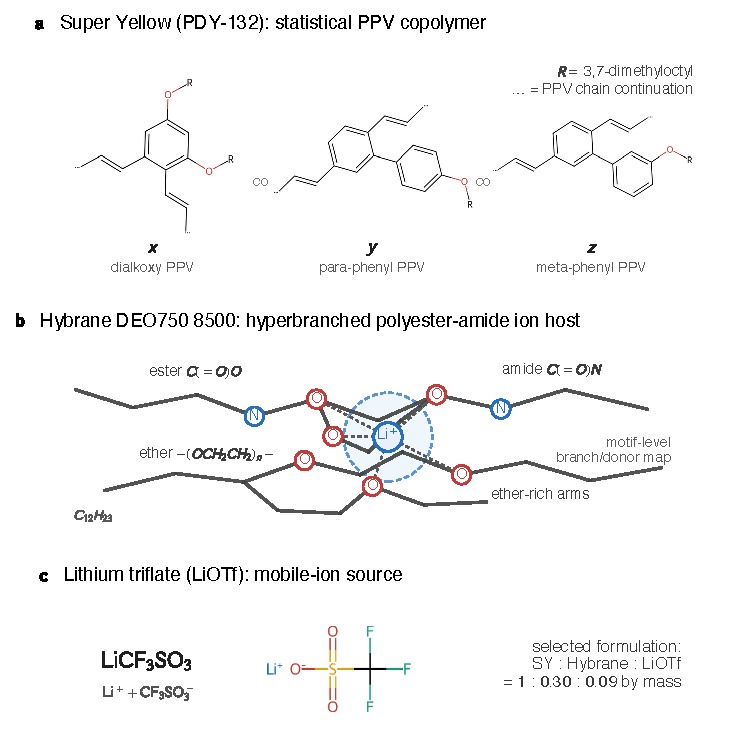
\includegraphics[width=\linewidth]{../figures/chapter2/composite_chemistry.pdf}
  \caption[Chemical components of the proof-of-concept composite]{Chemical components of the proof-of-concept composite. \textbf{(a)} \SY{} is the commercial PDY-132 PPV-family statistical copolymer; \(R\) denotes the branched 3,7-dimethyloctyl side chain. \textbf{(b)} \Hybrane{} DEO750 8500 is represented as an oxygen-rich hyperbranched polyester-amide motif, highlighting ether, ester, and amide donor sites rather than a monodisperse molecular formula. \textbf{(c)} \LiTf{} is shown as the lithium salt of triflate, \ce{LiCF3SO3}. The selected active-layer formulation is \SY{}:\Hybrane{}:\LiTf{} = 1:0.30:0.09 by mass.}
  \label{fig:ch2_si_composite_chemistry}
\end{figure}

\subsection{Solution Preparation and Film Deposition}

The three stock solutions were prepared separately in cyclohexanone at \SI{15}{\milli\gram\per\milli\litre} (\SY{}), \SI{10}{\milli\gram\per\milli\litre} (\Hybrane{}), and \SI{5}{\milli\gram\per\milli\litre} (\LiTf{}). The \SY{} solution was stirred at \SI{50}{\celsius} overnight. The solutions were then mixed to give the final mass ratio \SY{}:\Hybrane{}:\LiTf{} = 1:0.30:0.09, corresponding to final concentrations of \SI{8.72}{\milli\gram\per\milli\litre}, \SI{2.62}{\milli\gram\per\milli\litre}, and \SI{0.78}{\milli\gram\per\milli\litre}, respectively. Solution handling was performed under dry nitrogen to limit moisture uptake.

ITO-patterned glass substrates were ultrasonicated successively in aqueous Mucasol detergent solution, deionised water, and 2-propanol, each for \SI{15}{\minute}. After drying under nitrogen, substrates were transferred immediately into a nitrogen glovebox (oxygen and water below \SI{1}{ppm}). The active layer was spin-coated at \SI{2000}{\rpm} for \SI{60}{\second}, then annealed at \SI{75}{\celsius} for \SI{3}{\hour}. The anneal removes residual cyclohexanone, allows chain relaxation, and stabilises the mixed polymer-electrolyte morphology.

The top Ag electrode was thermally evaporated in the glovebox through a shadow mask defining the \SI{0.0825}{\square\centi\metre} junction. Ag was deposited at \SIrange{0.1}{0.5}{\nano\metre\per\second} to a total thickness of \SI{100}{\nano\metre}, monitored by quartz crystal microbalance. The slow initial rate was used to limit metal penetration into the soft polymer layer, which would otherwise risk filamentary shorts~\cite{Hung1997}.

\section{Electrical Protocol Detail}\label{app:ch2_electrical_protocols}

Electrical measurements used a Keithley 2450 SourceMeter connected to a custom probe station and controlled through Keithley TestScript Builder. Unless noted otherwise, measurements were carried out under nitrogen, with voltage applied to the Ag top electrode relative to the grounded ITO bottom electrode.

\subsection{Assay-to-Specimen Map}\label{app:ch2_assay_specimens}

The proof-of-concept claim concerns one formulation and device architecture, not one physical junction carrying every assay. \Cref{tab:ch2_assay_specimens} records the finest specimen identity recoverable from the local archive and the published supporting information. A crossbar ``junction'' or ``pixel'' is one ITO/active-layer/Ag overlap; several junctions share a fabricated substrate and therefore are not independent device or batch replicates.

\begin{table}[htbp]
  \centering
  \caption[Assay-to-specimen map for the proof-of-concept evidence]{Assay-to-specimen map for the Chapter 2 evidence. ``Published summary'' indicates that the numerical result is recoverable from Ref.~\cite{PradoSocorro2022}, but the local archive does not resolve the physical specimen identifier.}
  \label{tab:ch2_assay_specimens}
  \footnotesize
  \setlength{\tabcolsep}{3pt}
  \begin{tabularx}{\linewidth}{p{0.18\linewidth} p{0.28\linewidth} X}
    \toprule
    \textbf{Assay} & \textbf{Recovered evidence unit} & \textbf{Supported inference} \\
    \midrule
    I--V hysteresis & One junction, NM\_v025 & Representative analogue hysteresis of the common formulation; no population estimate. \\
    Pulse potentiation/depression & One junction (L5), NM\_v055 & Reversible pulse-protocol demonstration. \\
    Pulse-number response & Five junctions, NM\_v055, Day 8 & Within-substrate junction spread; not independent-device or batch reproducibility. \\
    STM/LTM retention & Three published fit traces; specimen ID unresolved & Existence and timescale of two protocol-defined retention regimes; no population estimate. \\
    EPSC state sequence & Published state ratios; specimen ID unresolved & Four-state protocol demonstration; no population estimate. \\
    STDP timing kernel & Five junctions, NM\_v055, Day 19 & Within-substrate mean timing response and junction spread. \\
    Shelf stability & Published time series; specimen roster unresolved & Calendar stability over the reported interval; not cycling endurance or batch stability. \\
    \bottomrule
  \end{tabularx}
\end{table}

\subsection{Read--Write--Wait Measurement}\label{app:ch2_read_write_wait}

The variable-pulse and variable-delay measurements use a common read--write--wait sequence (\cref{fig:stm_ltm}). First, a low reading pulse, \(V_{\mathrm{read}}=\SI{0.5}{\volt}\), establishes the initial conductance \(G_0\). This voltage is below the independently determined ionic-redistribution threshold of approximately \SI{0.7}{\volt}~\cite{PradoSocorro2022}. Second, a train of \(N_{\mathrm{pulses}}\) write pulses of duration \SI{0.1}{\second} perturbs the ionic configuration. Third, after a waiting time \(t_{\mathrm{wait}}\) under open-circuit conditions, a second read pulse measures \(G_f\). The reported response is \(\Delta G=(G_f/G_0)\times100\%\). Between experiments, the device was reset by shorting the junction for \SI{300}{\second}, and \(G_0\) was checked before the next measurement.

\begin{figure}[htbp]
  \centering
  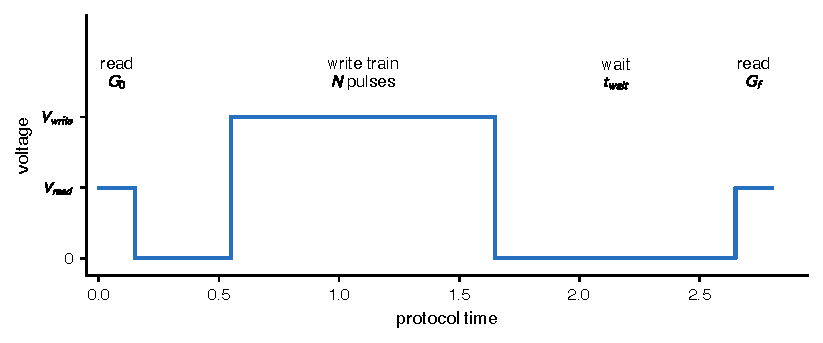
\includegraphics[width=0.82\linewidth]{../figures/chapter2/read_write_wait_protocol.pdf}
  \caption[Read--write--wait protocol]{Read--write--wait protocol used for the pulse-number and retention measurements. A low read pulse establishes \(G_0\), a train of write pulses perturbs the ionic configuration, a controlled open-circuit waiting time allows relaxation, and a second read pulse measures \(G_f\). Generated from the protocol reported in Ref.~\cite{PradoSocorro2022}.}
  \label{fig:stm_ltm}
\end{figure}

\subsection{Extended Synaptic Protocols}\label{app:ch2_extended_protocols}

The EPSC experiment defines states operationally by their signed current response under a common \SI{+1}{\volt} read-out bias. The device is first held at \SI{+1}{\volt} for \SI{1}{\second} to define \(S_0\). Two \SI{+2}{\volt}, \SI{50}{\milli\second} pulses generate excited states \(S_1\) and \(S_2\), and two \SI{-2.5}{\volt}, \SI{50}{\milli\second} pulses generate inhibitory states \(S_3\) and \(S_4\). The signed ratios \(R_n=I_{S_n}/I_{S_0}\) are reported in \cref{subsec:epsc}.

For STDP, pre- and postsynaptic spikes are emulated by triangular voltage waveforms applied to the two-terminal device. The experimentally applied voltage is the algebraic sum
\begin{equation}
  V_{\mathrm{device}}(t,\Delta t) = V_{\mathrm{pre}}(t) + V_{\mathrm{post}}(t-\Delta t),
\end{equation}
with \(\Delta t=t_{\mathrm{post}}-t_{\mathrm{pre}}\). Each signed spike template has maximum amplitude \(V_{sp}=\SI{1.55}{\volt}\) and duration \SI{1.2}{\second}; \(\Delta t\) was varied from \SI{-600}{\milli\second} to \SI{+600}{\milli\second}. Template overlap produces a measured resultant as large as \SI{3.1}{\volt} at $|\Delta t|=\SI{50}{\milli\second}$. Negative \(\Delta t\) produces potentiation and positive \(\Delta t\) produces depression under the sign convention used in \cref{subsec:stdp}. The applied-voltage logic of both protocols is shown in \cref{fig:ch2_si_extended_protocols}.

The archived branch-fit file is not used for the thesis figure because its depression curve does not fit the five-junction mean in the master table. Both branches were therefore re-fitted directly to that mean using the offset exponential of \cref{eq:stdp_fit}, excluding the zero-delay point. The resulting constants are \(\tau_{+}=\SI{89}{\milli\second}\) and \(\tau_{-}=\SI{150}{\milli\second}\); junction-resampling 95\% intervals are \SIrange{78}{95}{\milli\second} and \SIrange{134}{172}{\milli\second}. These intervals describe within-substrate junction variation only. The fitted parameters and audit metrics are recorded in \path{handouts/ch2_stdp_fit.csv} and regenerated by \path{scripts/ch2_figures.py}.

\begin{figure}[htbp]
  \centering
  \begin{subfigure}[t]{0.48\linewidth}
    \centering
    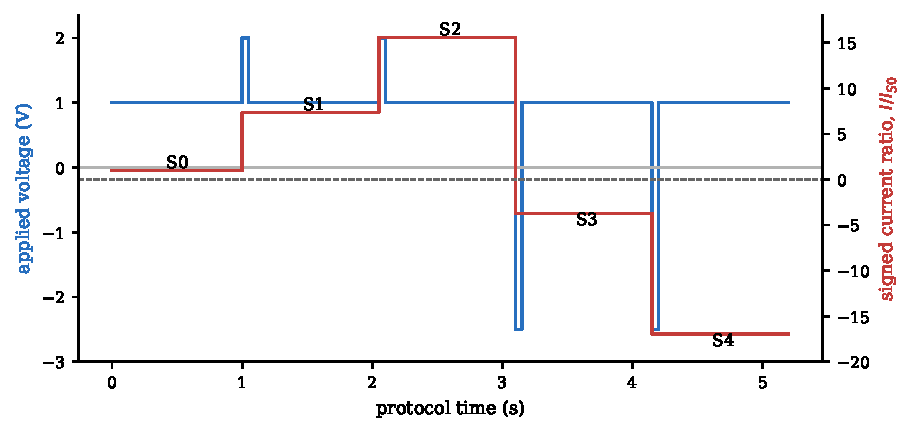
\includegraphics[width=\linewidth]{../figures/chapter2/full_epsc_trace.pdf}
    \caption{EPSC protocol trace.}
    \label{fig:ch2_si_epsc_trace}
  \end{subfigure}\hfill
  \begin{subfigure}[t]{0.48\linewidth}
    \centering
    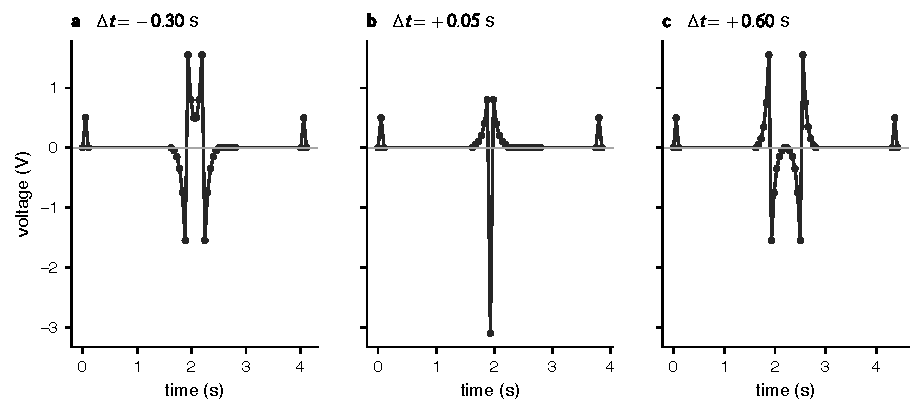
\includegraphics[width=\linewidth]{../figures/chapter2/stdp_waveforms.pdf}
    \caption{STDP waveform superposition.}
    \label{fig:ch2_si_stdp_waveforms}
  \end{subfigure}
  \caption[Extended EPSC and STDP supporting panels]{Supporting protocol panels for the extended synaptic measurements. \textbf{(a)} Reconstructed EPSC trace showing the applied-voltage sequence and the signed current ratios reported for states \(S_0\)--\(S_4\). \textbf{(b)} Measured total voltage across junction L5 for three timing offsets, read directly from the NM\_v055 Day19 archive. These panels document the protocol logic; the compact evidence used in the main chapter is reported in \cref{fig:extended_synapse_summary}.}
  \label{fig:ch2_si_extended_protocols}
\end{figure}

\subsection{Retention-Fit Parameters}\label{app:ch2_retention_fits}

\Cref{tab:ch2_retention_fit_parameters} lists the standard-exponential fit parameters reported for the proof-of-concept retention traces. The fits use \(G_f/G_0=R_\infty+A\exp(-t_{\mathrm{wait}}/\tau)\), with \(\beta=1\) fixed.

\begin{table}[htbp]
  \centering
  \caption[Published retention-fit parameters]{Published standard-exponential fit parameters for the Chapter 2 retention traces. No free stretch exponent, confidence interval, or goodness-of-fit statistic was reported for these proof-of-concept fits.}
  \label{tab:ch2_retention_fit_parameters}
  \begin{tabular}{llll}
    \toprule
    Condition & \(\tau\) (s) & \(R_\infty\) & \(A\) \\
    \midrule
    \SI{1}{\volt}, 10 pulses (STM) & 2.57 & 1.01 & 0.374 \\
    \SI{1}{\volt}, 50 pulses (STM) & 3.01 & 1.01 & 0.91 \\
    \SI{3}{\volt}, 10 pulses (LTM) & 4.73 & 1.05 & 3.30 \\
    \bottomrule
  \end{tabular}
\end{table}

\section{Morphology and Stability Support}\label{app:ch2_morphology_stability}

The spin speed was selected from a \SIrange{500}{3000}{\rpm} optimisation~\cite{PradoSocorro2022}. Low speeds produced films that were too thick and less uniform; high speeds made the film thin enough for substrate roughness to matter. The selected fabrication condition used \SI{2000}{\rpm}, giving a \SI{209}{\nano\metre} active layer measured by contact profilometry across a masked step edge with an Ambios XP-1 profilometer.

Surface topography was characterised by tapping-mode AFM using a Bruker Dimension Icon instrument, a silicon probe with resonant frequency \SI{300}{\kilo\hertz} and force constant \SI{40}{\newton\per\metre}, and a scan rate of \SI{0.6}{\hertz}. The AFM images showed smooth films with RMS roughness of \SIrange{1}{3}{\nano\metre} over the investigated spin-speed range~\cite{PradoSocorro2022}. The absence of large phase-separated features supports the reading of the active layer as a homogeneous polymer-electrolyte composite at the scale relevant to the vertical junction.

Ambient shelf stability was assessed for approximately two weeks (\(\sim\)\SI{300}{\hour}) on unencapsulated devices stored in air at room temperature~\cite{PradoSocorro2022}. The monitored quantities were baseline conductance \(G_0\), maximum conductance change \(\Delta G_{\mathrm{max}}\), and STM retention time \(\tau_S\). All three remained within \SI{20}{\percent} of their initial values over the measurement window. This is a shelf/calendar stability result, not a cycling-endurance measurement. \Cref{fig:ch2_si_morphology_stability} summarises the film thickness, AFM roughness, and shelf-stability metrics together.

\begin{figure}[htbp]
  \centering
  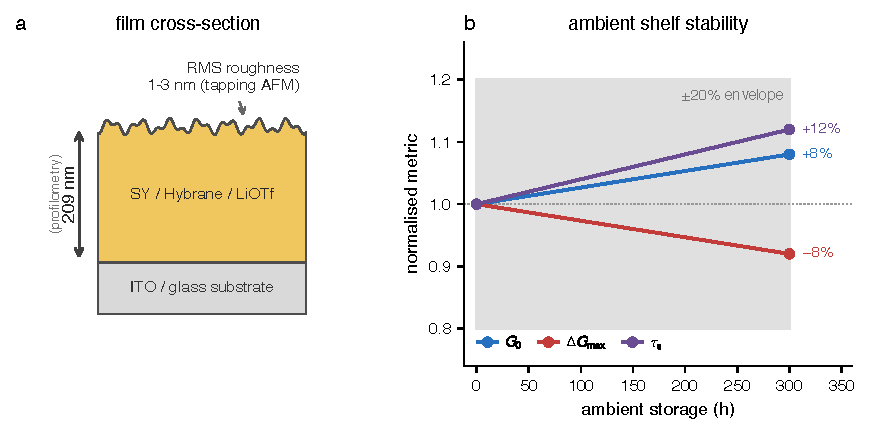
\includegraphics[width=\linewidth]{../figures/chapter2/morphology_stability_support.pdf}
  \caption[Morphology and shelf-stability support]{Supporting morphology and shelf-stability summary for the Chapter 2 device family. The selected processing condition gives a \SI{209}{\nano\metre} active layer; tapping-mode AFM reports \SIrange{1}{3}{\nano\metre} RMS roughness across the investigated spin-speed window; and the ambient shelf-stability metrics remain within a \SI{20}{\percent} envelope over approximately \SI{300}{\hour}. Compiled from the supporting measurements reported in Ref.~\cite{PradoSocorro2022}; this is not a cycling-endurance result.}
  \label{fig:ch2_si_morphology_stability}
\end{figure}

\paragraph{Encapsulation outlook.} The ambient stability is expected to improve further with encapsulation, standard practice in organic electronics: a thin \ce{SiO2} or \ce{Si3N4} barrier deposited by atomic-layer or chemical-vapour deposition would suppress the oxygen and water ingress that are the two primary degradation pathways~\cite{LewisWeaver2004}. That even unencapsulated devices survive two weeks establishes the baseline robustness of the composite.

\section{Ion-Transport Models for the Composite}\label{app:ch2_ion_models}

This section details the injection and bulk-transport descriptions summarised in \cref{sec:mechanism}. The two limiting-case models are inherited from the polymer light-emitting electrochemical cell (LEC) literature and reconciled by van~Reenen \textit{et al.}~\cite{vanReenen2010} as two regimes of the same ion redistribution.

\subsection{Equilibrium Ion Distribution and Response to an Applied Field}

In the idealised zero-bias starting state inherited from LEC models, the film is macroscopically electroneutral and any field is limited to built-in or interfacial contributions~\cite{Pei1995,deMello1998,vanReenen2010}. At the molecular scale, \ce{Li+} may occupy coordination environments in the Hybrane matrix and triflate may exist in free, paired, or aggregated states; those populations were not measured in this blend.

When a voltage is applied across the device, an electric field $\mathcal{E} = V/d$ (where $d$ is the film thickness) is established. In the absence of free charge carriers that could screen this field, it would be uniform throughout the film. However, the mobile ions respond to the field by migrating: cations drift toward the cathode (ITO at positive bias on Ag), and anions drift toward the anode (Ag). This migration leads to the build-up of a charged double layer at each electrode interface on a timescale determined by the ionic mobility and the film thickness. The resulting non-uniform ionic charge distribution concentrates the field in a thin screening length near each electrode, while the bulk of the film is field-free~\cite{deMello1998,deMello2002}, with consequences for charge injection described by the two models below.

\subsection{Electrodynamic Model}

In the electrodynamic (ED) model, first formulated by deMello \textit{et al.}~\cite{deMello1998, deMello2002} to describe LECs, charge injection at the electrode--organic interface is the rate-limiting step for current flow. In this injection-limited regime, the current density is governed by thermionic emission over the Schottky barrier at the metal--polymer interface,
\begin{equation}
  J \propto T^2 \exp\!\left(-\frac{\Phi_B}{k_B T}\right),
  \label{eq:thermionic}
\end{equation}
where $\Phi_B$ is the effective barrier height, $T$ the absolute temperature, and $k_B$ the Boltzmann constant. The ionic double layer at the electrode interface reduces $\Phi_B$ by bending the polymer bands: positive ionic charge near ITO lowers the conduction-band edge there, while negative ionic charge near Ag raises the valence-band edge, both reducing the effective injection barrier. In the memristive context, conductance changes therefore arise from changes in the interface ion concentration: a higher concentration of positive ions near ITO means lower $\Phi_B$, higher hole injection, and higher conductance, and the ions relax back toward equilibrium by thermal diffusion once the field is removed, the physical basis of the memory decay.

\subsection{Electrochemical Doping Model: Ohmic Injection}

The electrochemical doping (ECD) model, formulated by Pei \textit{et al.}~\cite{Pei1995} and developed by subsequent authors~\cite{Smith1997, Matyba2009}, instead takes charge injection to be ohmic (not rate-limiting), so the majority of the voltage drop occurs in the bulk and the current is limited by bulk conductivity. The defining feature is that ion accumulation \textit{electrochemically dopes} the conjugated polymer: cations accumulate near the cathode, stabilising injected electrons (\textit{n}-doping), and anions near the anode, stabilising injected holes (\textit{p}-doping); the doped regions are far more conductive than the undoped polymer. The degree of doping (and hence the conductance) is set by the extent of ionic migration, which is governed by the history of applied voltage, so the conductance records the cumulative ionic-displacement history.

\subsection{Resolution of the Two Models}

The prolonged LEC-community debate over the relative validity of the ED and ECD models was reconciled by van~Reenen \textit{et al.}~\cite{vanReenen2010}, who showed that the limiting behaviour depends on injection conditions: ED when injection is strongly barrier-limited and ECD when injection is closer to ohmic. A device may move between these limits as ionic redistribution develops. Applying that framework here is physically plausible, but the present measurements do not identify an ED-to-ECD transition or justify assigning ED uniquely to triflate and ECD uniquely to \ce{Li+}; \cref{sec:mechanism} states the assignment and its failed simple cation-ordering prediction explicitly.

\section{Historical Comparison at the Time of Publication}\label{app:ch2_comparison}

\Cref{tab:ch2_historical_comparison} places the device alongside representative organic and hybrid memristive devices available at the time of the 2022 publication, on the axes of \cref{subsec:memristive_metrics}: device structure, accessible conductance states, short- and long-term memory, STDP, and reversibility. It is a historical positioning, not a 2026 state-of-the-art claim.

\begin{sidewaystable}
  \centering
  \caption[Historical comparison with organic and hybrid memristive devices]{Historical comparison of key performance metrics of the present work with representative organic and hybrid memristive devices available at the time of the 2022 publication. ``2-T'' = two-terminal; ``3-T'' = three-terminal; ``STM'' = short-term memory; ``LTM'' = long-term memory; ``STDP'' = spike-timing dependent plasticity; ``---'' = not reported or not applicable.}\label{tab:ch2_historical_comparison}
  \footnotesize
  \setlength{\tabcolsep}{3pt}
  \begin{tabular}{llccllcc}
    \toprule
    \textbf{Reference} & \textbf{Material} & \textbf{Structure} & \textbf{States} & \textbf{STM} & \textbf{LTM} & \textbf{STDP} & \textbf{Reversible} \\
    \midrule
    Zakhidov 2010~\cite{Zakhidov2010}      & [Ru(bpy)$_3$]$^{2+}$/PF$_6^-$ & 2-T & 2    & ---           & ---        & No  & Partial \\
    Lei 2014~\cite{Lei2014}                & PVA film                  & 2-T & 2    & ---           & ---        & No  & No      \\
    Liu 2016~\cite{Liu2016}                & [EV(ClO$_4$)]/(BTPA-F)   & 2-T & cont.& Yes (tunable) & Yes        & No  & No      \\
    Gkoupidenis 2015~\cite{Gkoupidenis2015}& PEDOT:PSS (OECT)          & 3-T & cont.& Yes           & No         & Yes & Yes     \\
    Xu 2016~\cite{Xu2016}                  & PEDOT:PSS (OECT)          & 3-T & cont.& Yes           & Yes        & No  & Yes     \\
    Kim 2018~\cite{Kim2018}                & Elastic organic composite & 3-T & cont.& Yes           & No         & Yes & Yes     \\
    Goswami 2017~\cite{Goswami2017}        & Molecular switch          & 2-T & 2    & ---           & Yes        & No  & Yes     \\
    Seo 2019~\cite{Seo2019}                & P3HT organic FET          & 3-T & cont.& Yes           & No         & Yes & Yes     \\
    \midrule
    \textbf{This work}~\cite{PradoSocorro2022} & \textbf{SY/Hybrane/LiOTf}  & \textbf{2-T} & \textbf{cont.} & \textbf{Yes (10--15\,s)} & \textbf{Yes (>45\,s)} & \textbf{Yes} & \textbf{Full} \\
    \bottomrule
  \end{tabular}
\end{sidewaystable}

Two combinations not represented in the comparison set at the time stand out. The first is that the same 2-T formulation and architecture support both \STM{}- and \LTM{}-labelled regimes while remaining fully reversible. Of the prior reports, Liu and co-workers~\cite{Liu2016} comes closest, with tunable short- to long-term transitions in a 2-T structure; the redox route, however, modifies the active layer irreversibly at each cycle, precluding practical cyclic operation~\cite{Heremans2011}. The present platform reaches comparable \STM{}/\LTM{} functionality with full reversibility (conductance returns to \(G_0\) after the reset protocol). The second is STDP in a fully reversible 2-T architecture: the earlier organic STDP demonstrations~\cite{Gkoupidenis2015, Kim2018, Seo2019} were all 3-T with a gate supplying the timing rule, whereas here the rule emerges from the superposition of pre- and postsynaptic pulses at the Ag terminal.

The remaining axes summarise the operating regime rather than a competitive claim. The ambient shelf lifetime (about \SI{300}{\hour} unencapsulated) exceeds most comparable unencapsulated organic memristive devices by roughly an order of magnitude~\cite{Shih2016}; cycling endurance, not characterised here, is where mature inorganic platforms reach \(>10^{10}\) cycles~\cite{IelminiWong2018}. Recalculation from the archived positive-pulse waveform gives \SIrange{0.084}{1.55}{\micro\joule} per event as the junction potentiates (median \SI{1.08}{\micro\joule}), higher than the picojoule budgets of dedicated CMOS neuromorphic hardware~\cite{IndiveriLiu2015,Horowitz2014} and mature inorganic memristors~\cite{YangStrukovStewart2013}. The large junction area and long pulse contribute, but proportional energy scaling with area has not been demonstrated and is not claimed.
